\chapter{Campaign Items and Resources} \label{resources}

\section{Book of Celestas}

\subsection{Introduction}

On the cover of the book it is written "The Book of Celestas. Blessed are the Celestials." The book is broken up like the Bible into different chapters. There are no verses though, just book names and then writings. The book contains prophetic messages, historical writings, letters, songs, sayings, instructions, and more. Here are some short summaries and important passages from a few of the books. This book can be given to the players after finding the prior or parts of it can be found from others. They can either obtain a whole book of Celestas (and then have to uncover it when they take time to sit and read) or they can be read parts of it from NPCs. 

\subsection{Origin}

In the beginning, The Celestials created the Heavens and the Planets. A singularity of reality from whence space was formed, energy was made, and time unraveled. A trinity of reality to be seen forever. From the dust of the ground, all species were made by Them and spread by Them across the cosmos. And as dust, only containing the power of dust. Each with a form of its own but with potential of ascension. Though none comparing to the power of Them.

With a promise of power and nature to assist, They guide those of lower to reach the path of enlightenment. Hallowed are the Celestials.

\subsection{Celestial decree}

Truth is the beginning of the Path and from Truth They exist. Blessed are those that deliver us from evil. For the followers are blessed and to greatness they will ascend. The followers walk in unity and by the laws they are led. Hallowed are those who walk in unison. 

Fear not the Celestials, fear the darkness that would conceal the knowledge of the universe. Believe in the Truth of all things, and you too may find the Path to enlightenment. Let not the darkness of the infinite universe dismay you. Through Darkness the Celestials exist, as for through Darkness the universe exists. The light of corruption spots the sky like the boils of a plague. Let the vastness of the Dark prove the truth of the Celestials. Blessed are those who follow the Path of Celestas. 

Glorious are the Celestials, who didst lead us to salvation, who did fight the evil that would doom us to mortal sin. Did they defeat the old spirits and cast them out? And now, with the strength of our will, they do call upon us to prevail against the corruption of all unbelievers. Guide us on the Path so that we may triumph over the enemy of our salvation and be with you in the End of Ends on the planes of enlightenment. Through the vast Darkness, the Celestials will blot out the falsehood of the stars. 

\subsection{Aroden}

Aroden then took off the mask and revealed his face. 'Your appearance matters not,' he said. 'Only the truth of spirit in your heart'. As born of the ugly, he followed the Celestials with all his heart and soul. To him it was gifted to be a prior, and a prophet among his people he became. Now it came to pass in the latter days of Aroden, that and Angel of the Celestials appeared to him, in the form of the Ether of his dreams. And a vision came upon Aroden. And it was seen that a large boulder came tumbling down a cliff side upon a spotless sheep and damaged the unborn flock. Due to the grace of the Celestials, the sheep lit with the aura of the sea and was raised in health and wellness to its former self. 

\subsection{Divine Instructions}

Lessons of days gone by teach us what will come to pass.  From the smallest seed of doubt springs forth the mighty poisonous tree of evil. Therefore, doubt must be purged, and only those pure to the Celestials can be permitted. Those turned from the knowledge and goal of the ascension must be purged.

\subsection{Ether}

The only true evil lives in the hearts of those who do not follow the Path. Otherwise, there is always some measure of brightness. And where there is light, the Celestials see all! But where there is Darkness, the Celestials have dominion over. For it is given to the mortals to live among the light, but to be among the Ascended is to be among the infinite. 

\subsection{Toldath of Gigikei}

This is the genealogy of the great Wanderer, Gigikei. He had six sons and one daughter. Gigikei of Kamelot born of the Island of Castiana, left his home at the age of thirty-five. He was a devout believer and followed the Celestials fervently. By this They blessed him with strength and that of a task to seek a far away treasure. Gigikei left the home of the Celestials and went into the unknown vastness of the sea. Through his generations of searching, he married seven times and had seven children, one with each wife. His children were diverse and spread across the four corners of Orilla. 

In the times of his old age, Gigikei had found a forest of majestic features. He concluded it could be nothing other than a special creation of the Celestials. He wandered this region for months until finally he came upon a stone door, appearing as though an entrance. When camping here at night, a dream fell upon him. In his dream, a Celestial being came to him and uttered the words “Et claritas tenebris ad ostium et urget.” Then he awoke and spoke the words he had dreamed to the stone. Then the door began opening before him. 

These are the children of Gigikei. Of them, none were taught the ways of the celestials by their father. The firstborn was Proclira, who became a hunter of spirits. Because he did not learn the ways of the Celestials, he and his people struggled to find their ways. They found strife within their families and the Celestials allowed this. 

Another was Taonishta, who became a sailor of the seas. He and his people spread far and wide and settled cities throughout Orilla and the Celestials allowed this. 
Another was Vegonbron, who became a keeper of the dead. He and his people created many temples and spread hidden treasures throughout the southern regions. They did not spread far but built a great city that they dwelt in and the Celestials allowed this. 

Another was Nibiron who became a holy man of false gods. Another, was Sahin and was a messenger of false prophets and teachings. These men learned the lifestyles of falsehood and found strife among their neighbors. They spread their false words among others and the Celestials allowed this.
The youngest of the brothers was Zebon, who was a troublemaker. He and his people existed throughout the areas of the others. The Celestials allowed this.

Of these six, the two holy men displeased the Celestials the most but they still allowed their actions. The Celestials allowed these things to come to pass so that in the day of the Lamb, They can use their false ways to teach the world Their power and Truth.

The daughter of Gigikei was Abydiss, who had many children and multiplied to a great number of people. The Celestials allowed this because one day, they would be removed from life in a twinkling of the eye for their false beliefs as a show of what the true Path is to follow. These are the descendants of Gigikei who were allowed to spread across the seas to some day be joined back into the Celestial Family.
It came to pass that after decades of multiplying, near the ends of their lives, the children of Gigikei learned of their relations and banded together in search for their father. They wandered into the Pluvian realm where they had found the same majestic features as Gigikei. From his great journey, the children were warned by their surroundings but eventually lost in time, and all but forgotten by their descendants. Never to find their father, for they were seeking not after the Truth of the Celestials, but after the false hopes of carnal pleasures.

\subsection{Markon}

So, it came to pass that Ver Omesh was gripped by a great famine. So Markon went to the Prophet Articus and asked to go to the forest for food. The prophet bade him be patient, for the Celestials provide for all who have faith. But Markon did not believe. So, the prophet drew a line in the sand and told him, 'Step across and you may do as you wish.' So Markon did and left the village and feasted on wild berries. The fruit was bitter. It did not satisfy him. He longed to return to the village but found that the line had widened to a great chasm. He called out to the Prophet in fear, but the Prophet said, 'The line has not changed; it is you who have changed. Step across if you truly believe.' So Markon prayed for forgiveness and took the first step. And the hands of the Celestials enveloped all those who welcomed him back. 

\subsection{Petrias}

As he lay there, dying in the sun, the sands of the desert all around him. In his delusion, Petrias imagined a great beast trotting across the sand of the sea. On the beast was a small Lamb, without blemish and of prime age. The Lamb had dominion over the beast and came to Petrias. The Lamb appeared divine in nature and spoke saying “By the power of Celestus, faith can save you.” He perceived this Lamb as the daughter of the Celestials. But in that moment, the Lamb and the beast vanished into darkness. Petrias spoke to a rock, not with his lips, but with his mind. And the rock wept tears of fresh water, and his thirst was quenched. Find the reward of doing right, in right. The reward of following the Celestials can be seen by following the Celestials. For in great devotion comes great blessings.

\subsection{Amica}

Amica was forgiven his transgression and found his way back to the Path. For he let unbelievers sway his beliefs and strayed from the Path. Through the herem of the unbelievers, his faith was shown true and he was restored to his rightful Path. Due to the faith that Amica believed with, the Celestials granted him with the powers of foresight and prophesizing.

It came to pass, that in the night of a storm a deep slumber came upon Amica. A vision came upon him which pictured a flock of sheep, and one spotless sheep which was birthing its young. When the firstborn of the flock had been fully removed, an angel of the celestials came and took it up to the heavens. At that instant, the Shepheard of the flock and all of the sheep that remained began to turn young and eventually collapse to nothing. And then it happened, that a great bolt of lightning struck the house of Amica, and it was burned up. By this he knew that this vision was a prophecy of times by the Celestials.
   
At the end of his life, through dedicated service and prostration all the days of his life, he had ascended as to a Celestial. Forever existing and eternally powered, he now watches over as an angel in the shadows.

\subsection{Aphorisms}

\textit{Caelium videri esset. Et terra rus ad sidera tollere vultus. Ex uno disce omnes.}

Auf Celestii as heaven was seen. And the countryside will lift its face to the stars. From one, all will learn.

\textit{Enim lupin purnum pravus intus.}

Auf Celestii as verily, the corrupted sinner will be cleansed from within.

\textit{Sanctus Celesti.}

Auf Celestii as Holy Celestials.

\textit{In fine mundi falsa et agnus pascent et elucentis fidei foci.}

Auf Celestii as in the end of the false world, the Lamb will rule with radiant faith.

\subsection{Toldath of Andras}

Andras chose to hunt the lion and was eaten by his prey. When instead become the surrounding he must have. Like a shadow blending in perfect. The followers of Celestas must put on perfection, and blend like a shadow. And when sin shines bright they must blot it out and grow to an infinite cloud, blotting out the shine of the stars. As the vast Darkness of Celestas encompasses the universe, so is the infinite potential of the followers.

And at the death of Andras, he had only three children. The firstborn of Seth was begotten when Andras was only twenty years old, in his prime. As an elder man of forty-five, the same year he was eaten by his prey, he conceived of the eternal twins, Ephraim and Manasseh. In Andras’ last moment, an angel visited him revealing this to him and revealed to him also that “on these two heirs will be built the foundation of all of the Celestial prophets.” From this moment to the end, all prophets of the Celestials will follow the bloodline of the eternal twins.

And within the following centuries, Ephraim and Manasseh were fruitful and multiplied. And a great nation was descended from them. These two men were great warriors but at a youthful age they both vanished into the great Pluvian forest and have not been seen or heard of since. 

\subsection{Tyolus}

And then did Tyolus say to the people of the low plains, 'Seek not the wickedness amongst your neighbors, lest it find purchase in your own house'. And he preached to the city of Barbosius and the townsfolk marveled. At the end of the fourth day, they all turned to believers of the Celestials and rose up against the neighboring villages who refused to believe. The Celestials blessed the people of Barbosuis with great strength and might and they were able to utterly destroy the unbelievers. In this the Celestials were pleased and blessed the people for years to come. And it came to pass that Tyolus was made a great prophet among the people of the region and set about to convert the whole Island in which he presided. 

Tyolus was a gifted prophet of the Celestials and given the gifts of divination and foresight. Through a great trance, he was given a vision. And he looked, and behold a pale Lamb descended from the heavens. Its coat was spotless and small. And this Lamb was gifted to a shepherd to be cared for. And in that moment the Lamb grew into a fine sheep and the trees and fields all blossomed in an instant. Then a toothless wolf came quickly and grabbed the sheep from the field. The wolf took the sheep in its mouth without harm and ran off into the distance with it. The weather outside was fierce and Tyolus awoke to the sound of a tree falling nearby. In that moment he knew that he had been gifted with a great vision from the Celestials.

\subsection{Beltachadzer}

Let not the words of deceivers lead you to doubt, nor the enticements they offer cause you to stray. For the unbelievers only exist to sway the followers from the teachings of Celestas. As a test of faith, they were formed of matter, so that the true followers will understand the importance of their following. And those who choose disobedience will be stripped away the chance at ascension, and forever be removed from existence. And those who are prideful and refuse to bow down, shall be laid low and made into dust. 

Just as Beltachadzer was corrupted and tried to lead astray the followers, others live to preach lies and pose as false prophets. Even through apparent wonders and signs from false gods, the teachings of the false will only lead to false hope. By fire Beltachadzer was destroyed and his soul removed from the promise of ascension.

\subsection{Ascension}

The flames of ignorance burn without pain. Beware the power or it will consume you before you know.

\subsection{Avernakis}

Life and death, light and darkness, despair and hope. The rift was created, and on that day, the Celestials were born. But the hatred of those who strayed from the true Path festered and bloomed in the dim corners of the Avernakis to which they have been cast! And consumed by this hatred, they poisoned all they touched, bringing death, suffering and despair. And the souls of their victims knew no peace, until the Celestials came and whispered to them: 'Sleep, for the end draws near!' And on that day, all will rejoice, when the Celestials come and lay them low. 

It is we who must seek the Truth of the universe in order to achieve enlightenment. There is only one Truth, Darkness is infinite.

\subsection{Infinite Pathway}

Blessed are the true believers, for only they shall walk the Path, and they shall be welcomed unto the realm of the Celestials and made as one with Them. Make yourself one with the Path, and the journey will lead you to eternity. Just as Darkness lives in eternity, so will the followers of Celestas be made.
Our journey towards enlightenment may take us to many unexpected places. When doubts and fears arise, look towards the promise of the Celestials. For with infinite subjugation comes infinite blessings. Ours is not to question, but to rejoice in Their service, for the Celestials are perfection. 

Leave not the smallest pebble, for any hindrance will slow the people's progress.  Pity not the blind man, for he is hindered not by the visions of this world. But rather, pity yourselves, for he shall see the light before you. For the Darkness that he sees contains more vastness than all the light of the unseen universe. Where we come from and where we are going are all the same. 

He spoke to the sky and said: 'And the people shall deliver the wicked unto your divine judgment, where their sins shall be weighed in the balance of all that is just and true'. Enemies of the Celestials will show no mercy in their attempts to lead us astray from the true Path, likewise we must attack with all the Strength with which we have been given. 

Those who abandon the Path are evil. Foolhardy are those who do not follow the Path. Those who reach enlightenment shall rejoice with the Celestials forever. The power and the greatness of the Celestials cannot be denied. Those who reject the Path to enlightenment must be destroyed. Those who seek the Path to enlightenment must not be led astray. Those who follow the Path of righteousness shall be raised up high. 

\subsection{Revelation}

Death is only the beginning of the real journey. Truth eludes he who does not seek it with both eyes wide. Paraphrased by Adria as Truth is elusive to those who refuse to see it with both eyes wide. Through salvation the blessings of Celestas are gifted. At the end of a life, when the ascension is reached, there is glory and honor magnified by the stars of the sky. As death comes like a thief in the night, the time for repentance and prostration cannot be delayed, for the gift of ascension will not come without hasty dedication.

In the time of the end, the beginning will start. The end of the corrupt and beginning of the bright shine of Celestus. The Lamb of the Celestials will bring power unending on the plain of the people. And in that day, the priors of Celestia will perform miracles of resurrection and wonders among the multitudes of the people, turning their hearts to the Truth and to righteous repentance and devotion. The Truth of the Celestials will spread across all of existence and all those who oppose will be purged for the good of their souls. She will bring fourth justice and remove all those who could stand in the way. The Celestials will give power to the followers so that none can defy, and She will light the way with an ever-burning radiance. The unbelievers will be removed, and peace and justice will rein in all places. The Lamb of Celestia will be shielded with the power of faith and Truth and none shall penetrate Her will.	



\subsection{Unique Items}

\begin{itemize}
	\item Pokeball: Captures 1 non-sentient being. Must succeed a hit roll at disadvantage. Creature must fail a DC10 wisdom save.
	\item Circlet of Instant Transmission (orange circlet with a gem in the middle. Writings on the side that says "This circlet contains the power of the Yardrat"): When placing two fingers (pointer finger and middle finger) on the center gem, the wearer will be instantly transported to a location they are looking at within 60 yards. The circlet contains 3 markings which represent three uses they can use, each with a 24 hour cooldown.
	\item Ring of Kaio-Ken (Silver ring with a red/orange sphere gem that glows with a fiery aura): Activated by saying "Kaio-Ken". The user takes twice as much damage and deals twice the damage. Takes half the user's level worth of HP damage per round of combat.
	\item Kamehameha Gauntlets (Blue Gloves with Goku symbol on them): Fires a blue beam of energy doing 1d12 damage per charge turn. Has a 2 hour cd raised to the power of how many charge turns were used (2$^\textrm{turns}$ hours CD). Must be used like a kamehameha from Dragonball z.
	\item Power Pole: Unbreakable pole that can extend up to 100 feet.
	\item Broly Bracelet (armbands): Adds +5 strength to the wearer but every round of combat they must save a DC17 Wisdom save or go berserk until succeeding the save. 
\end{itemize}

\subsection{Weapons}

\begin{itemize}
	\item Excalibur
	\item Frostmourne
	\item The Master Sword
	\item The Z-Sword
	\item Adamantium Gauntlet
	\item Scorpion chain
	\item Stars of Guiden (throwing stars)
	\item Blades of Chaos
	\item Bido's Boomerang
	\item Sting
	\item Staff of the white wizard
\end{itemize}

\subsection{Color Chart}

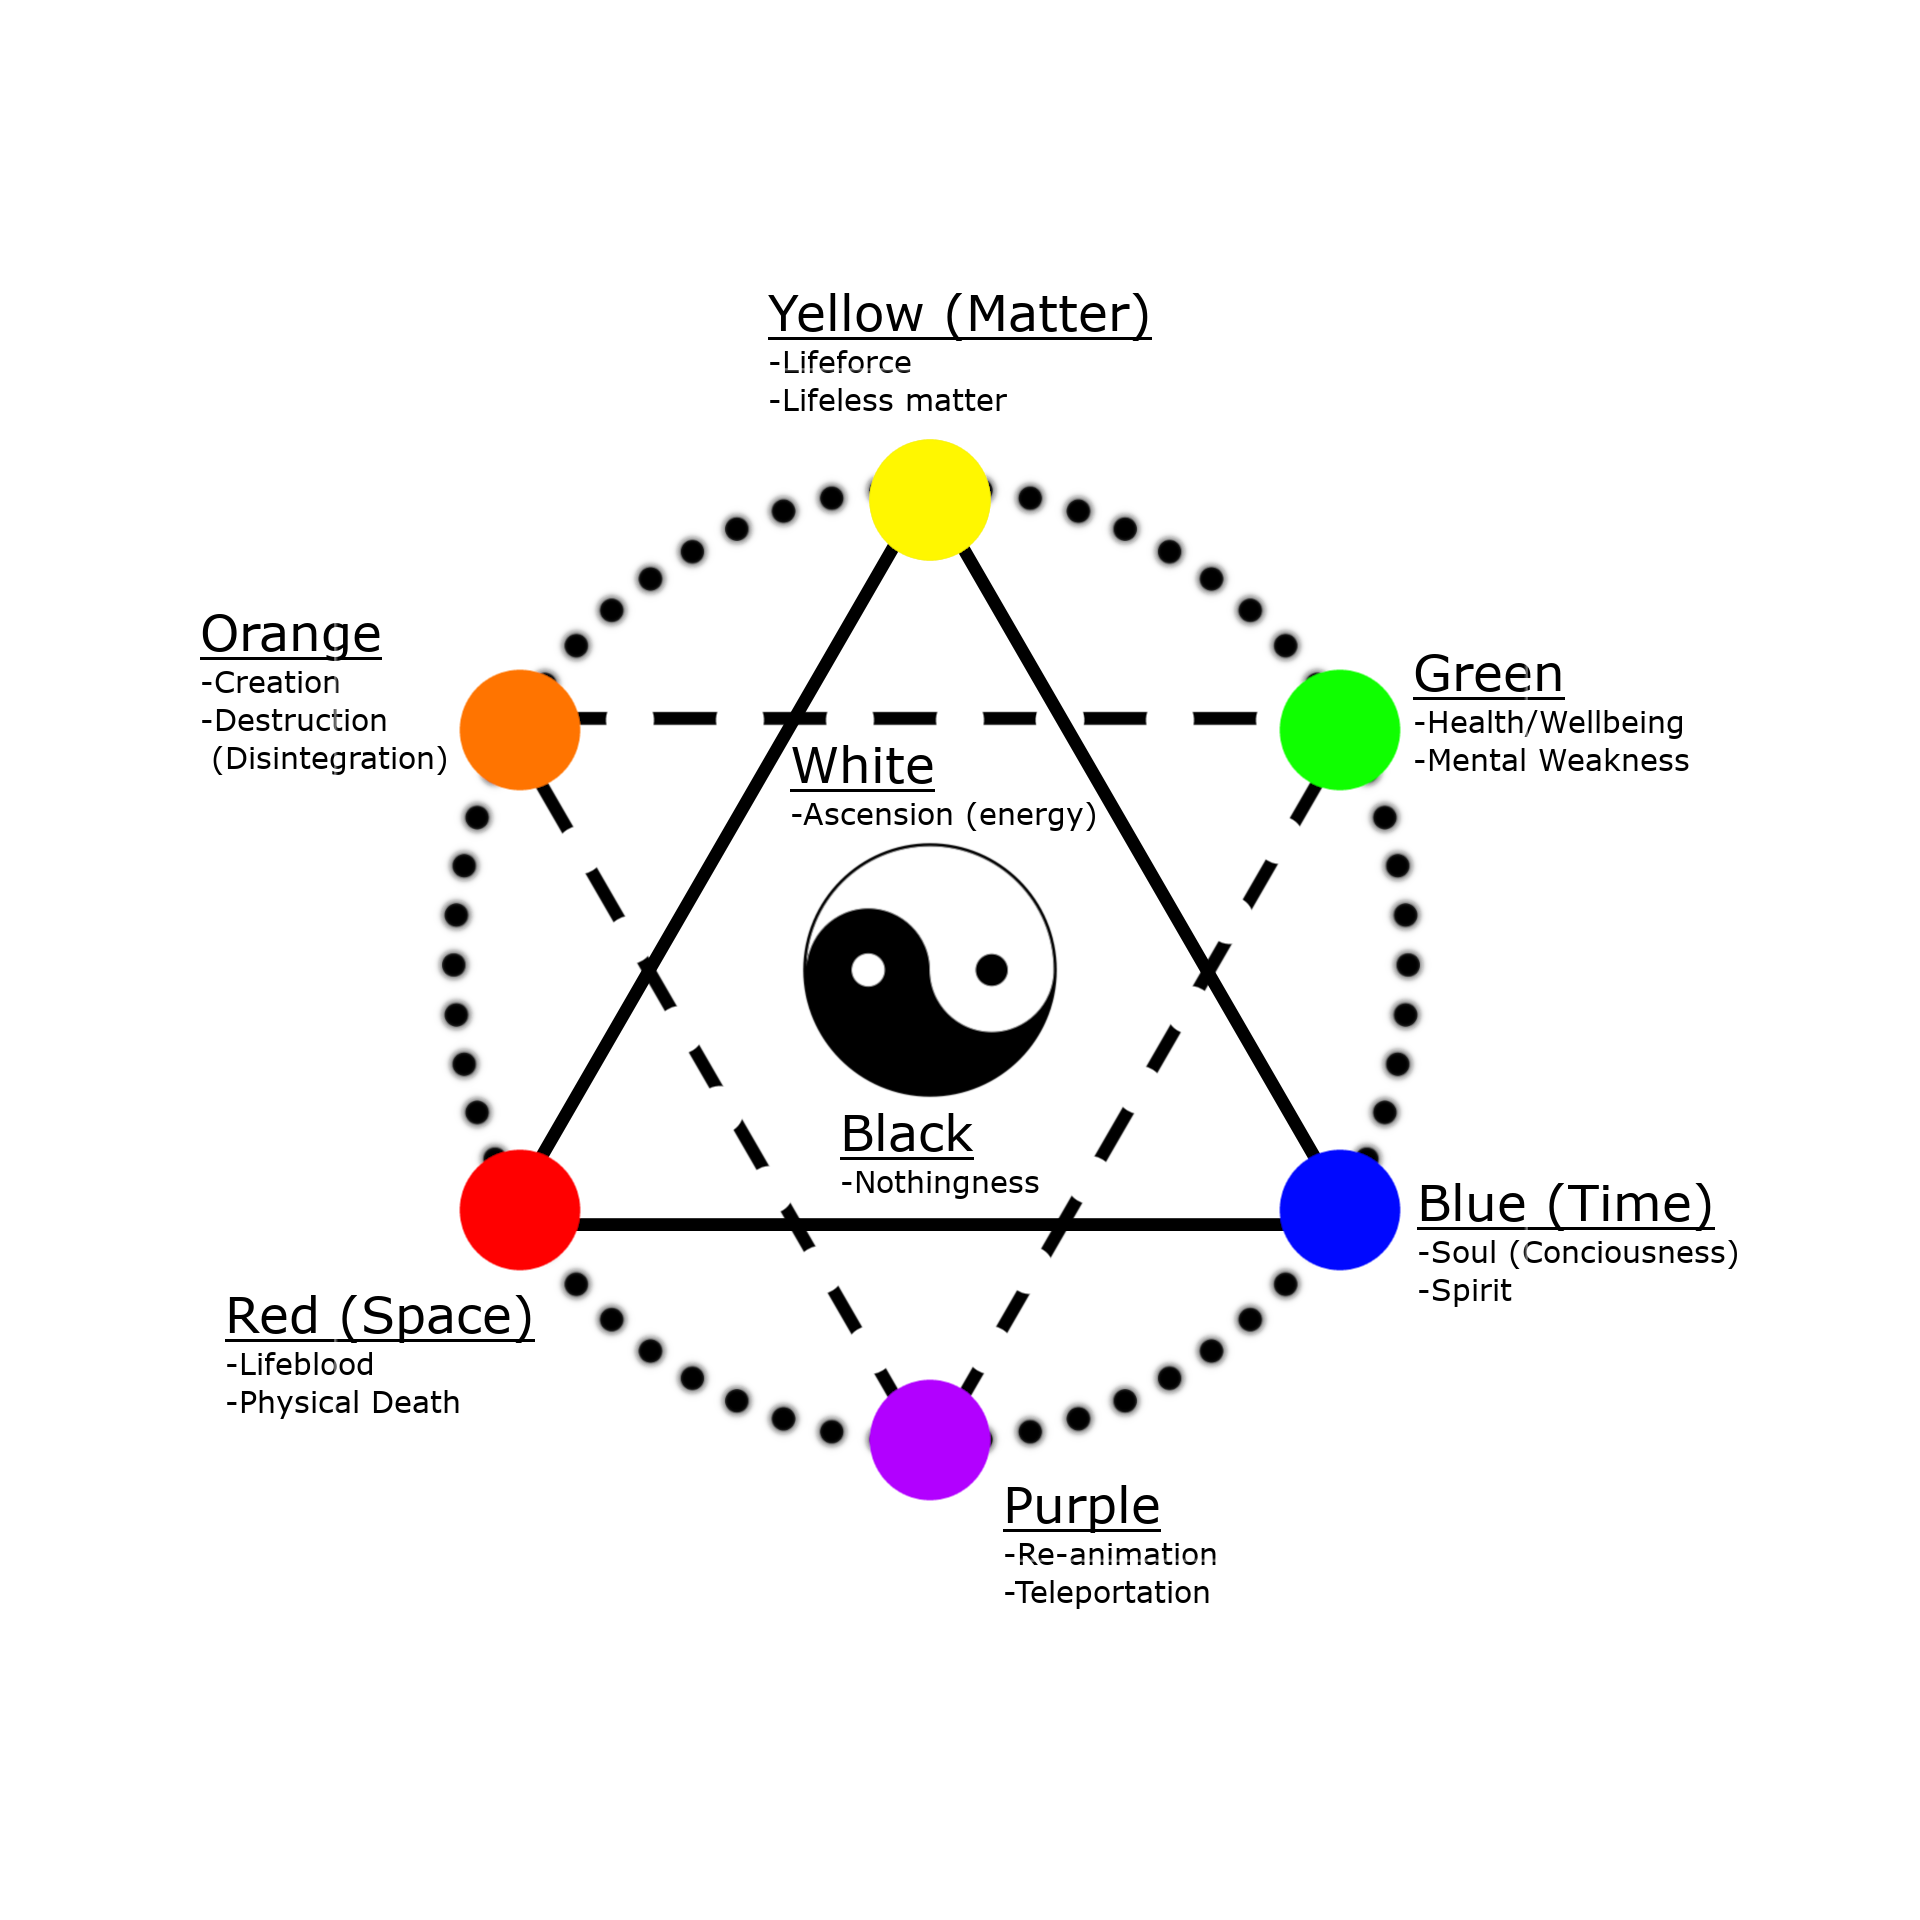
\includegraphics[width=\linewidth]{img/ColorChart.png}

\subsection{Campaign Names For NPCs}

\begin{multicols}{4}
	\begin{itemize}
		\item Nero
		\item Artemisia
		\item Neokoros = temple sweeper'
		\item Saturninus
		\item Quirinius
		\item Sentius
		\item Lysanias
		\item Rabbi Akiba
		\item Bar-Kokhba
		\item Mishnah
		\item Flavius
		\item Tiberias
		\item Claudius
		\item Helena
		\item Ekron
		\item Samaria
		\item Hattush
		\item Rehum
		\item Iddo
		\item Bilgah
		\item Sallu
		\item Sully
		\item Gizmo
		\item Amok
		\item Ezra
		\item Xerxes
		\item Haggai
		\item Roshak
		\item Matthgar
		\item Nattiee
		\item Nugs
		\item Endovelicous
		\item Adalia
	\end{itemize}
\end{multicols}